\section{Desenvolvimento da solução}

O desenvolvimento da solução para o projeto foi um processo que envolveu várias etapas que foram estabelecidas
com o tempo. Desta forma a solução foi sendo adaptada conforme os novos requisitos.
O desenvolvimento não só envolveu componente software como também hardware, o que levou com que o desenvolvimento do
protocolo em ambiente laboratorial fosse essencial para garantir a eficácia do sistema. Como houve parte do desenvolvimento
que foi realizada fora do laboratório, também foi desenvolvido uma componente que simula o hardware implementado.
A solução teve em conta não só a usibilidade do mesmo, como também as dificuldades e limitações encontradas durante o processo de 
desenvolvimento.


\subsection{Requisitos}

Nesta secção irão ser identificados todos os requesitos funcionais e não funcionais estabelecidos ao longo do estágio:

\begin{itemize}
    \item[] Requisitos funcionais:
        \begin{itemize}
            \item Leitura de dados de temperatura: O estagiário deverá desenvolver um sistema de leitura de dados de temperatura; 
            \item Interface gráfica: A solução deve constar com uma interface gráfica que permitirá ao usuário controlar o teste;
            \item Vizualização dos dados obtidos em tempo real: o sistema densenvolvido deve permitir ao usuário visualizar os dados obtidos do 
            teste em tempo real;
            \item Base de dados: Todos os valores obtidos do teste devem ser guardados numa base de dados local;
            \item Comunicação: O sistema deve suba guardar a comunicação entre os dispositivos (entre a RPI e o EVSE e entre a RPI e o MainPC).
        \end{itemize}
    \item[] Requisitos não funcionais:
        \begin{itemize}
            \item Desempenho: O sistema deve ser capaz de processar dados em tempo real sem atrasos significativos;
            \item Escalabilidade: O sistema deve ser capaz de suportar um aumento no volume de dados sem comprometer o desempenho;
            \item Reabilidade: O sistema deve garantir a integridade e a disponibilidade dos dados durante a operação;
            \item Segurança: O sistema deve garantir o padrão mínimo de segurança dos dados e a proteção contra acessos não autorizados;
            \item Manutenibilidade: O sistema deve ser projetado para facilitar a manutenção e atualização ao longo do tempo.
        \end{itemize}
    \item[] Restrições:
        \begin{itemize}
            \item Todo o sistema desenvolvido deve estar limitado ao material e recursos disponíveis no laboratório;
            \item O sistema deve ser testado em ambiente laboratorial para garantir fidelidade dos resultados;
            \item O sistema deve ser capaz de operar em diferentes ambientes sem perder a sua funcionalidade.
        \end{itemize}
\end{itemize}
    
    

\subsection{Arquitetura e tecnologias}

Ao longo do estágio, enumeras tecnologias e arquiteturas foram levadas em conta para corresponder aos requesitos do Cliente. Como os requesitos foram mudando ao longo do projeto, a estrutura do projeto acabou por ser ajustada.
Nesta secção irão ser aboradadas as diferentes arquiteturas e tecnologias abordadas e os seus motivos para serem (ou não) selecionadas.

\subsubsection{Componentes de hardware}
Os componentes de hardware utilizados foram lemitados à disponibilidade de recursos e materiais no laboratório. Para a implementação da solução foram
utilizados uma Raspberry Pi 3 e 4 sensores DS18B20.

Para a validação do protocolo, foi utilizado um carregador EVSE desenvolvido pelo Laboratório e uma câmara termal (incubadora) IMP 400 da HERATERM 
(disponível no Laboratório).

A Raspberry Pi 3 é um microcomputador de baixo custo e alta versatilidade, ideal para projetos de prototipagem e automação. Outra vantagem é a sua capacidade de se conectar a diversos dispositivos e sensores, facilitando a integração em projetos de IoT.
Foi instalado na RPI o sistema operacional Raspbian, que fornece uma interface amigável e suporte a diversas bibliotecas necessárias para o desenvolvimento do projeto, nomeadamente um conjunto de drives e configurações para utilizar a entrada GPIO da Raspberry.
A entrada GPIO foi essencial para a comunicação entre os sensores DS18B20 e a Raspberry Pi, permitindo a leitura e o controle dos dispositivos conectados. 
Outra vantagem da Raspberry é a integração de uma placa de rede no sistema, o que facilitou na comunicação com outros dispositivos e a troca de dados entre eles.
Para toda a configuração e estabelecimento da comunicação entre os dispositivos, foi utilizado o livro \cite{Molloy_2016}.

Os sensores DS18B20 são utilizados para medir a temperatura e são conectados à Raspberry Pi através da entrada GPIO, permitindo a leitura precisa dos dados de temperatura. Foi selecionado este sensor, pelos seguintes motivos:
\begin{itemize}
    \item Versatibilidade: O sensor apresenta um fio comprido o que ajuda no posicionamento dos sensores dentro da câmera termal.
    Além disso o sensor é encapsolado, o que o torna resistente a ambientes adversos.
    \item Leitura da temperatura digitalmente: A entrada GPIO da RPI só lê valores digitais e não valores analógicos (muito comum em sensores de temperatura). O sensor DS18B20 lê a temperatura digitalmente, o que facilita na obtensão dos dados (não necessita de um módulo analógico).
    \item Custo: Os sensores são acessíveis e disponíveis no mercado.
\end{itemize}

O carregador EVSE desenvolvido pelo INESCTEC é um carregador AC (alternate current), 
monofásio (230VAC), Potência nominal dos carregadores = 7.4kW ~= 32A, que tem instalado
diversos sensores que permitem medir valores de corrente, tensão, frequência e temperatura 
(os valores de temperatura remetem ao circuito). Pelo fato de ler tensão e corrente, pode-se 
calcular potência e o consumo de potência (W) no tempo nos da o consumo ou então, carregamento em energia (W/h),
o que é essencial para ver a eficiência do carregamento do carro elétrico ao longo do tempo.
Dentro do carregador tem uma Raspberry Pi que faz o gerenciamento de controle do carregamento e 
possibilita a comunicação do EVSE com uma base de dados do INESC para envio dos dados de carregamento.


A IMP 400 é uma câmara termal que permite controlar a temperatura interna, garantindo condições controladas para a realização dos testes. 
Tem a capacidade de manter a temperatura interna constante entre os 5°C e os 70°C (o que acaba por 
abranger o intervalo de temperaturas sentidas em Portugal). Internamente ela possui uma sensor de temperatura
que permite saber a temperatura da câmara durante do teste. Por fim, a câmara termal possui ainda
uma entrada RS 232 que permite a comunicaçao serial port com a Raspberry Pi. Devido a uma limitação
da própria câmara termal, apenas comandos de querry estão disponíveis (permite por exemplo obter a temperatura
do sensor interno da própria câmara), mas comandos de set (por exemplo alterar a temperatura da câmara) não estão disponíveis.
Para uma melhor compreensão sobre as funcionalidades da câmara termal foi utilizada o seu manual \cite{chamber_manual} e para questões mais específicas a equipa de suporte da HERATERM.

Além disso, também foram utilizados outros componentes como resistências, cabos e conectores para garantir
a comunicação entre os dispositivos e a Raspberry Pi.

\subsubsection{Componentes de software}

Os componentes de software utilizados foram os principais alvos no estudo de arquiteturas e tecnologias. O sistema desenvolvido é composto por um conjunto 
de módulos que trabalham em conjunto para garantir a funcionalidade do sistema. Os principais componentes de software utilizados foram: 
\begin{itemize}
    \item[.] Sistema Operacional: O sistema operacional utilizado na RPI foi o Raspbian, 
    que é uma distribuição do Linux otimizada para a Raspberry Pi. O Raspbian fornece 
    uma interface amigável e suporte a diversas bibliotecas necessárias para o 
    desenvolvimento do projeto;
    \item[.] Linguagem de Programação: A linguagem de programação utilizada foi o Python, 
    que é amplamente utilizada em projetos de automação e IoT devido à sua simplicidade 
    e versatilidade. O Python possui diversas bibliotecas que facilitam a comunicação 
    com os sensores e a manipulação dos dados obtidos;
    \item[.] Base de Dados: Para armazenar os dados obtidos dos sensores, foi utilizado 
    o MySQL, que é um sistema de gerencimento de base de dados relacional amplamente
    utilizado. O MySQL foi escolhido devido à sua robustez, escalabilidade e facilidade de uso,
    além de ser compatível com o Python através da biblioteca MySQL Connector. Outro fator
    importante é facto de ser o principal sistema de base de dados utilizado no laboratório,
    o que facilitou a integração com outros sistemas já existentes;
    \item[.] Interface Gráfica: Para criar a interface gráfica do sistema, foi utilizada a 
    biblioteca PyQt, que é uma biblioteca de desenvolvimento de interfaces gráficas para Python;
    \item[.] Dashboard: Para a visualização dos dados obtidos em tempo real, foi utilizado o Grafana,
    uma plataforma de visualização de dados que permite criar dashboards interativas e personalizadas open source.
    \item[.] Bootstrapping: Para garantir a inicialização correta do sistema, foi utilizado o
    assemble para a instalação e configuração dos componentes de software necessários na RPI e dockerfile
    com integração devcontainer no MainPC.
\end{itemize}

Além destes componentes, foram ainda utilizados outros softwares que ajudaram no desenvolvimento do
protocolo, nomeadamente:
\begin{itemize}
    \item[.] Git: Para o controle de versão do código-fonte e facilitar o envio de ficheiros do computador de desenvolvimento para a RPI;
    \item[.] Visual Studio Code: Como IDE para o desenvolvimento do código-fonte;
    \item[.] MySQL Workbench: Para a gestão da base de dados MySQL, permitindo a criação e 
    manipulação de tabelas, consultas e outros objetos das bases de dados;
    \item[.] RealVNC: Para o acesso remoto à Raspberry Pi, permitindo a visualização e controlo da 
    interface gráfica do sistema a partir de outro computador;
    \item[.] Drawio e Mermaid: Para a criação de diagramas que ajudam na visualização da 
    arquitetura do sistema e no planeamento do projeto;
    \item[.] Fritzing: Software de prototipagem eletrónica que foi utilizado para desenhar o circuito de ligação dos sensores DS18B20 à Raspberry Pi,
    facilitando a compreensão do circuito e a sua implementação.
\end{itemize}

\subsection{Solução desenvolvida}

Um teste de temperatura corresponde a um processo de obtenção de dados de temperatura durante um período de tempo
que podem apresentar características como a temperatura inicial da câmara termal e a temperatura final da mesma. 
O protocolo tem como objetivo principal garantir as condições necessárias para a realização do teste de temperatura,
além de ter em conta outros fatores como a comunicação entre os dispositivos, a leitura dos dados dos sensores e a 
visualização dos dados obtidos.

Para ajudar na interpretação dos dados obtidos do teste, foi utilizado Mean Absolute Error (MAE) e Root Mean Square Error (RMSE)
para calcular o instante onde a temperatura lida pelo sensor de controlo da câmara termal e o sensor de controlo estabilizaram.

A solução desenvolvida pode ser dividida em duas componentes principais: 
\begin{itemize}
    \item[.] \textbf{RPI}: Corresponde à parte do sistema que é responsável por controlar os sensores de temperatura DS18B20,
    obter os dados de temperatura da câmara termal e do EVSE e comunicar com o MainPC sobre o estado
    do teste;
    \item[.] \textbf{MainPC}: Corresponde à parte do sistema que é responsável por servir de interface
    para o usuário, através de uma interface gráfica. Além disso é responsável por comunicar com
    a RPI sobre as ações a serem realizadas, como iniciar ou parar o teste. É no MainPC que está
    instalado uma dashboard (Grafana) que permite visualizar os dados obtidos em tempo real e uma base de dados (MySQL)
    que armazena os dados obtidos do teste.
\end{itemize} 

Ambas as componentes têm uma base de dados MySQL que armazena os dados obtidos do teste, 
permitindo a consulta e análise posterior dos dados. O schema de ambas as bases de dados 
é o mesmo. Para conseguir ver os resultados obtidos em tempo real, ambas as componentes 
têm um sistema de migração de dados através de schedulling. Para tal ser possível, a comunicação
entre a RPI e o MainPC é essencial.

Todos subsistemas estão integradas com paralelismo via threads, o que permite que as diferentes 
componentes do sistema possam funcionar de forma independente e simultânea, além de ser fácil de 
desativá-las via .env. No MainPC é ainda utilizado sinais (via pyqtSignal) para a thread da 
interface gráfica comunicar com as restantes threads do MainPC. 

Desta forma, o esquema do protocolo pode ser traduzido no seguinte diagrama:
\begin{figure}[H]
    \centering
    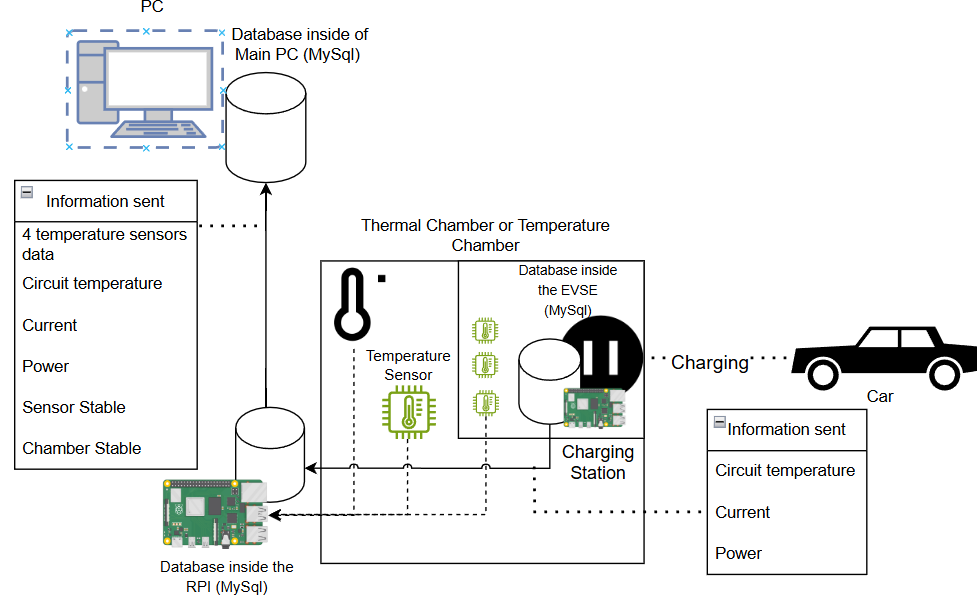
\includegraphics[width=0.8\textwidth]{figures/protocol_diagram.png}
    \caption{Diagrama do protocolo de comunicação entre a RPI e o MainPC}
    \label{fig:diagrama_protocolo}
\end{figure}

Nas próximas secções, serão abordadas as diferentes componentes essenciais do sistema, assim
como sua instalação.

Outro ponto importante a ter em conta é que o sistema é modular, que permite facilmente desativar
features, alterar configurações (IP's, portas, etc.) e alterar parâmetros. Para tal, foi utilizados
ficheiros .env que permitem definir as variáveis de ambiente do sistema, facilitando a configuração.
Mais informações sobre podem ser encontradas na documentação geral do protocolo [DOCUMENTAÇÃO].

\subsubsection{Sensores de temperatura DS18B20 e circuito}

Para a leitura dos dados de temperatura dos sensores DS18B20, foi desenvolvido um circuito que permite a 
conexão dos sensores à Raspberry Pi através da entrada GPIO. Como o circuito é possível de ser 
soldado, permite uma maior robustez e fiabilidade na conexão dos sensores.

\begin{figure}[H]
    \centering
    \begin{minipage}{0.6\textwidth}
        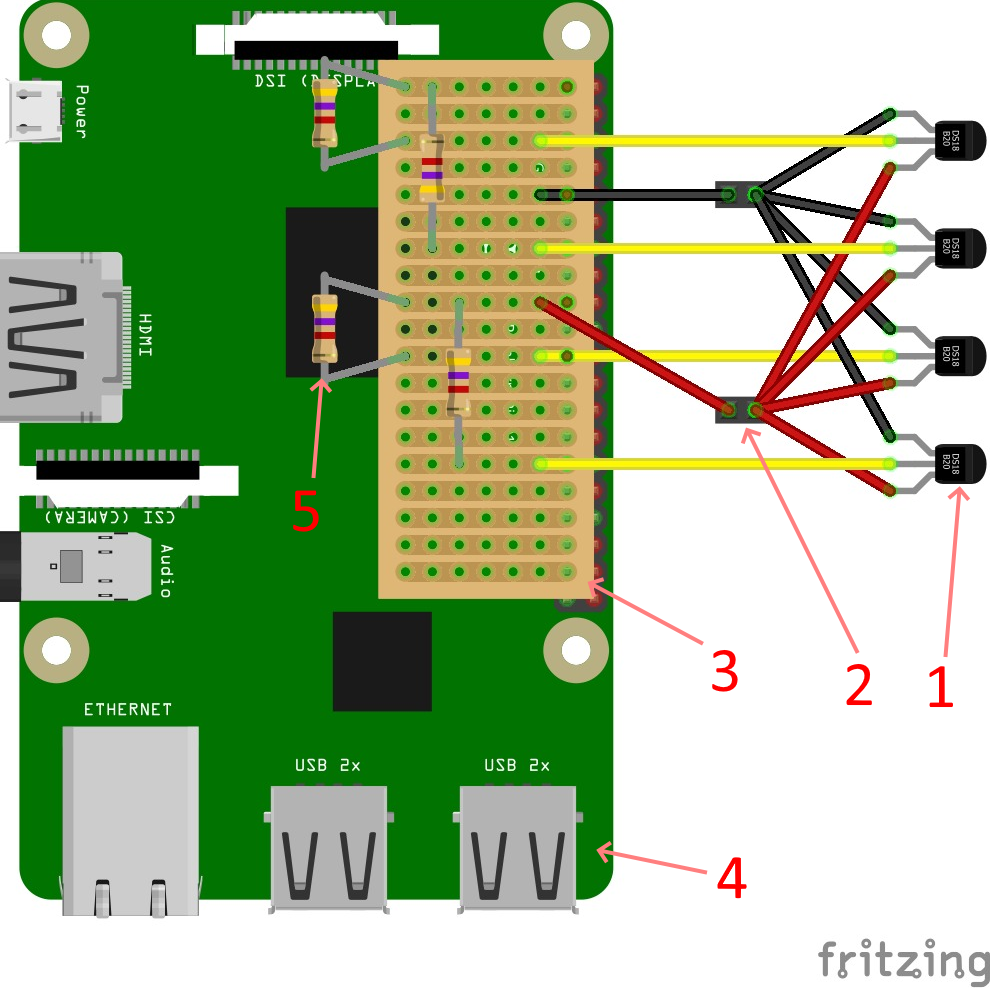
\includegraphics[width=\linewidth]{figures/circuit_dig.png}
    \end{minipage}%
    \hfill
    \begin{minipage}{0.35\textwidth}
        \small
        \textbf{Legenda:}
        \begin{enumerate}
            \item Sensor DS18B20 
            \item Conector
            \item Busboard de ligação
            \item RPI
            \item Resistência de $4.7\,\mathrm{k}\Omega$
        \end{enumerate}
    \end{minipage}
    \caption{Diagrama do circuito de ligação dos sensores DS18B20 à RPI}
    \label{fig:circuit_dig}
\end{figure}

\begin{figure}[H]
    \centering
    \begin{minipage}{0.48\textwidth}
        \centering
        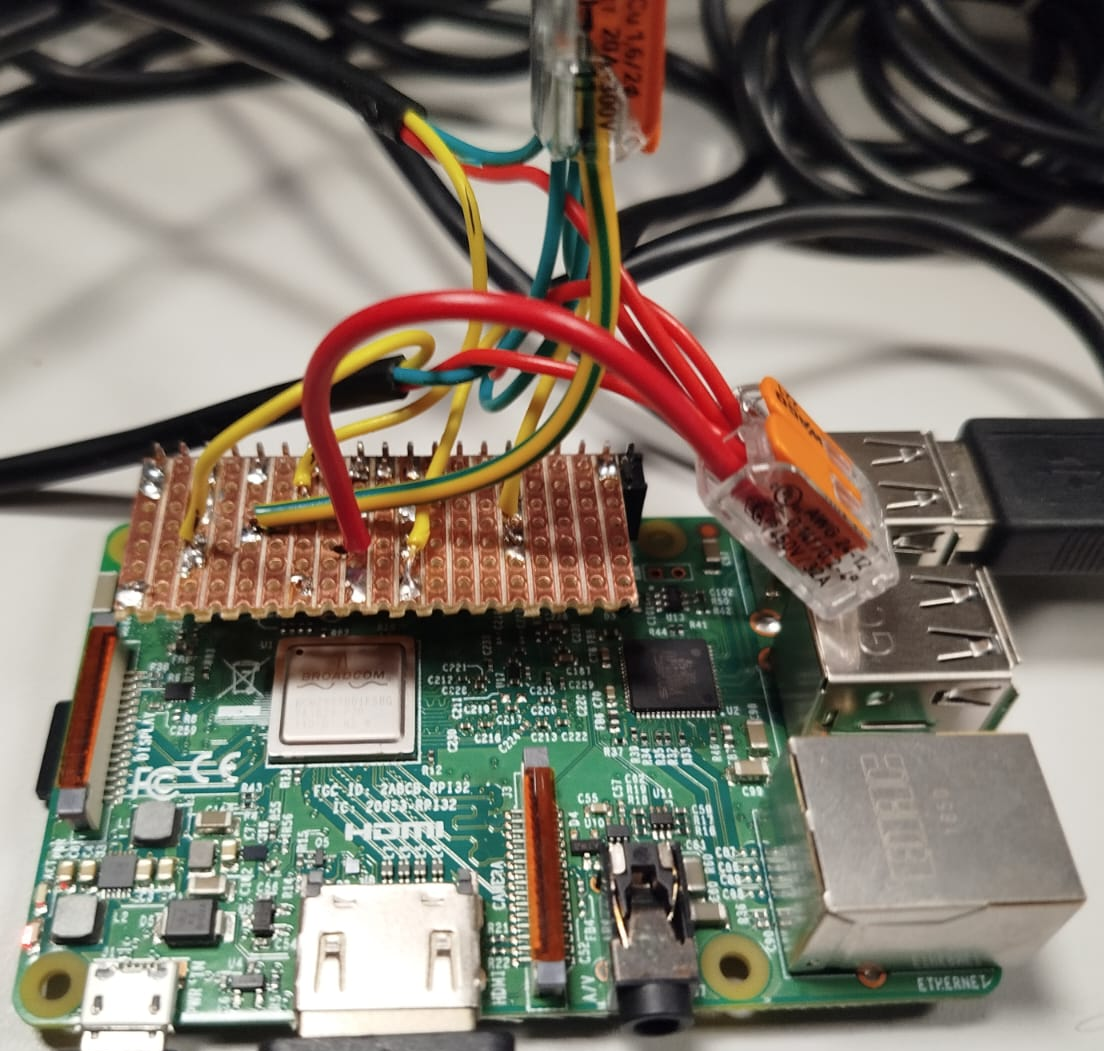
\includegraphics[width=\linewidth]{figures/circuit_1.png}
        \caption{Vista de cima do circuito de ligação dos sensores DS18B20 à RPI}
        \label{fig:circuit_1}
    \end{minipage}\hfill
    \begin{minipage}{0.48\textwidth}
        \centering
        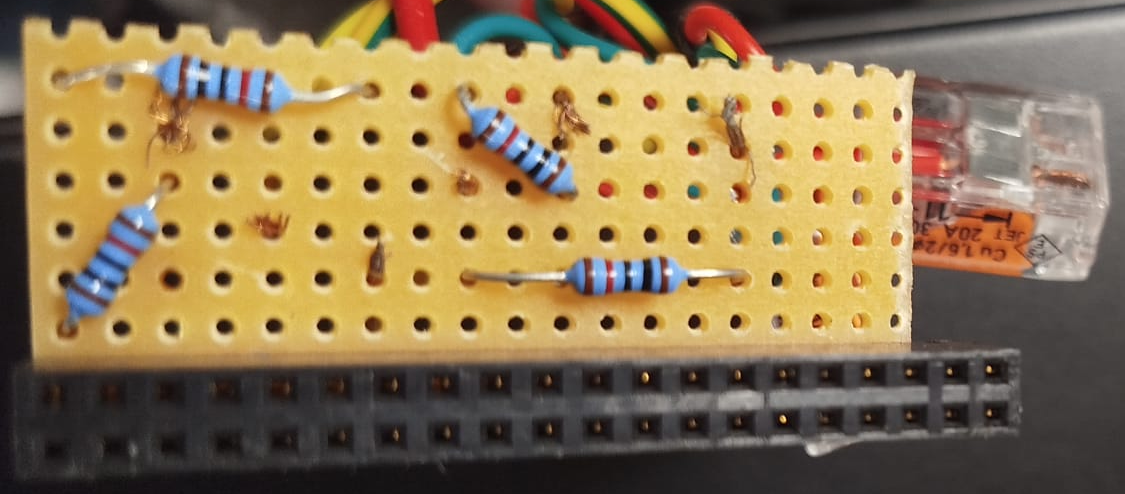
\includegraphics[width=\linewidth]{figures/circuit_2.png}
        \caption{Vista das resistências do circuito de ligação dos sensores DS18B20 à RPI}
        \label{fig:circuit_2}
    \end{minipage}
\end{figure}


Este circuito permite a conexão de mais sensores, contudo decidimos apenas instalar 4 sensores DS18B20,
um dos sensores é utilizado para medir a temperatura da câmara termal (servindo como controlo da temperatura
da câmara) e os outros três são posicionados no interior do EVSE em diferentes locais, para medir a temperatura
do carregador em diferentes pontos.

Para a sua implementação de hardware e software (leitura dos sensores), foi utilizada os sites 
\cite{Brian_Mark_Benoit_Santos_Alessandro_2023} e \cite{Campbell_2025}, a datasheet do sensor DS18B20 \cite{ds_datasheet}.



\subsubsection{Interface gráfica}

A interface gráfica foi desenvolvida utilizando a biblioteca PyQt e tem como objetivo principal
ajudar o utilizador a controlar o teste de temperatura, permitindo criar (estabelecer tempo, temperatura
do teste e descrição do teste), iniciar o teste de temperatura, parar o teste forçadamente e prolongar 
a duração do teste. A interface foi desenvolvida para ser fácil de implementar outras funcionalidades
no futuro.

\begin{figure}[H]
    \centering
    \begin{minipage}{0.6\textwidth}
        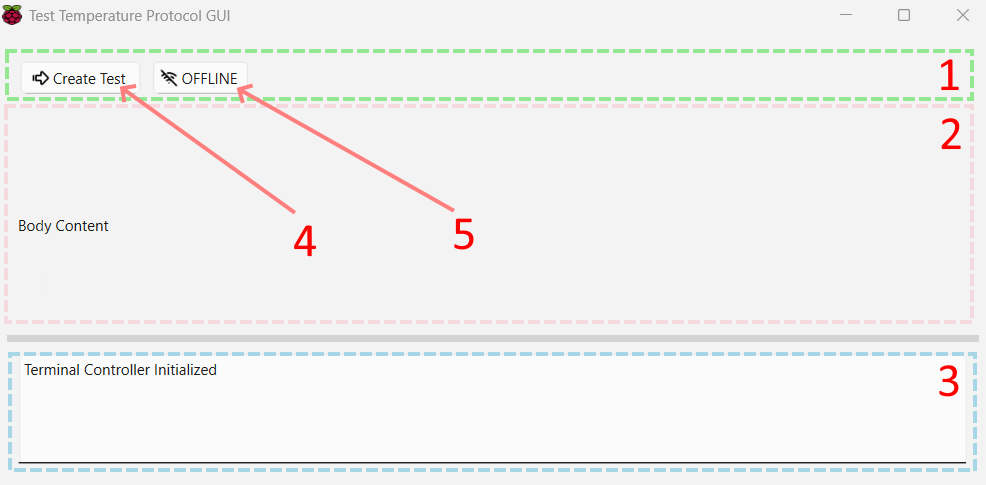
\includegraphics[width=\linewidth]{figures/gui_1.png}
    \end{minipage}%
    \hfill
    \begin{minipage}{0.35\textwidth}
        \small
        \textbf{Legenda:}
        \begin{enumerate}
            \item Upbar
            \item Body
            \item Terminal
            \item Botão de Create a Test
            \item Botão de conecção com a RPI
        \end{enumerate}
    \end{minipage}
    \caption{Interface gráfica do protocolo}
    \label{fig:gui_1}
\end{figure}

O butão Connection permite ao utilizador estabelecer a conexão com a RPI (com os parametros de IP e porta definidos no ficheiro .env).
Após a conexão ser estabelecida, o utilizador pode criar um teste de temperatura, através do botão Create a Test, apararecendo
em pop-up a janela ().

\begin{figure}[H]
    \centering
    \begin{minipage}{0.6\textwidth}
        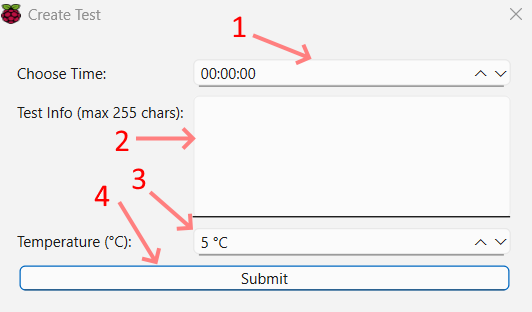
\includegraphics[width=\linewidth]{figures/gui_2.png}
    \end{minipage}%
    \hfill
    \begin{minipage}{0.35\textwidth}
        \small
        \textbf{Legenda:}
        \begin{enumerate}
            \item Cronometro do teste
            \item Descrição do teste
            \item Temperatura do teste
            \item Botão de submissão do teste
        \end{enumerate}
    \end{minipage}
    \caption{Pop Up de criação de um teste de temperatura}
    \label{fig:gui_2}
\end{figure}

Se o formulário for preenchido corretamente (o tempo do teste ser maior que 0), o teste é criado 
comunicado para a RPI (dos sensores DS18B20). Mais informações sobre o processo de comunicação
em \autoref{sec:comunicacao}.

Para comunicar as interações do utilizador com as outras threads do MainPC (comunicação e schedulling), foi utilizado
o pyqtSignal (nativo do PyQt), que permite enviar sinais entre as diferentes threads do MainPC.

\subsubsection{Comunicação}     \label{sec:comunicacao}

A comunicação entre os dois dispositivos é essencial para a criação/controlo dos testes de temperatura,
mas como também principal via para manter a sicronização do sistema de schedule dos dois dispositivos (MainPC e RPI). 
Também ajuda para notificar o sistema schedule do MainPC quando o sensor de controlo e o sensor da câmara termal estabilizaram.

A comunicação entre a RPI e o MainPC é feita através de um protocolo SSL/TLS para garantir a
segurança dos dados transmitidos. Para tal existe a necessidade de criar um certificado SSL/TLS
que é utilizado para estabelecer a conexão segura entre os dois dispositivos.

Apesar da comunicação funcionar peer to peer, para facilitar a implementação a RPI comporta-se como
um servidor (abre uma porta onde espera por uma conexão) e o MainPC como um cliente (conecta-se à RPI).
Após a conexão ser estabelecida, e a autenticação por certificados validada a RPI não aceita mais nenhuma
conexão, acabando por estabelecer um sistema peer to peer.


\begin{figure}[H]
    \centering
    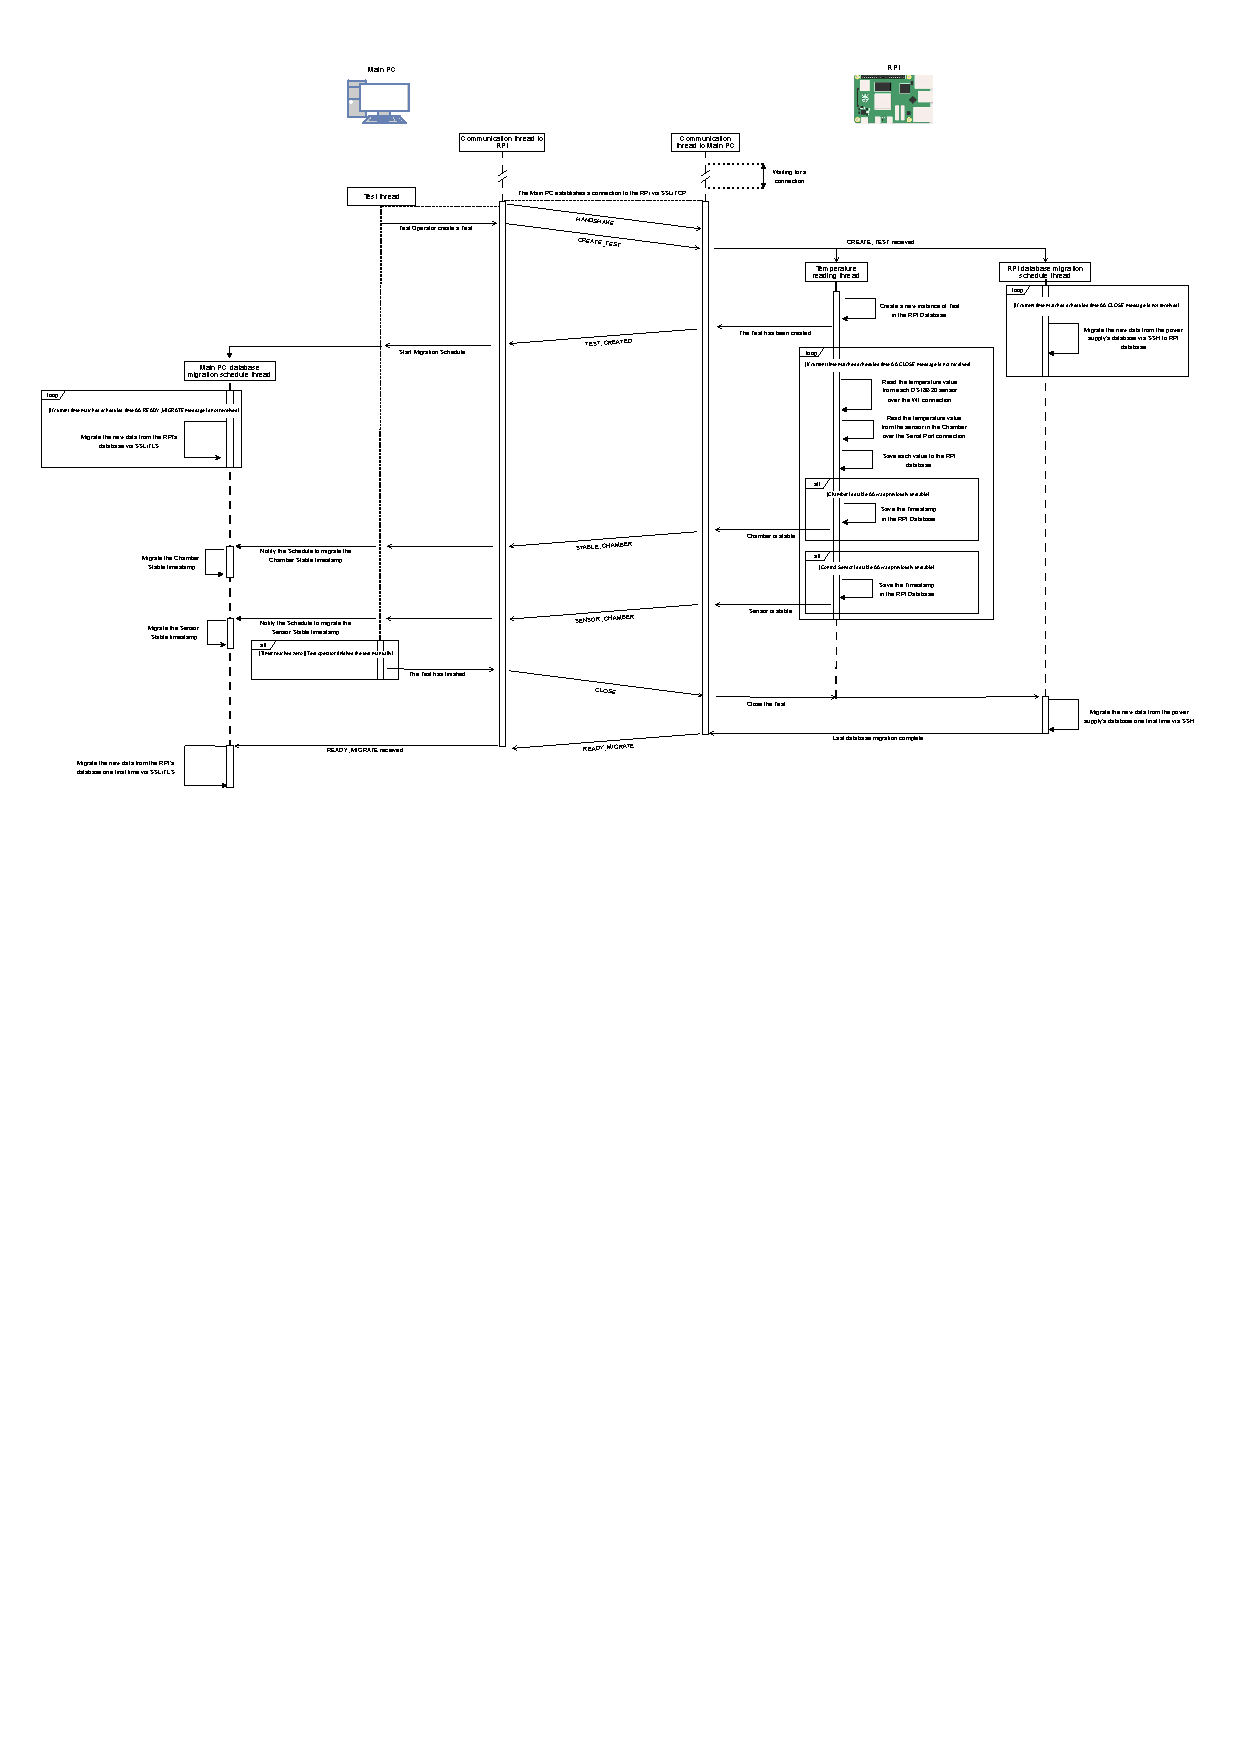
\includegraphics[width=\textwidth, clip, trim=0 16cm 0 0]{figures/communication.pdf}
    \caption{Diagrama do protocolo de comunicação entre a RPI e o MainPC}
    \label{fig:diagrama_comunicacao}
\end{figure}

Mais informações sobre o processo de comunicação entre a RPI e o MainPC podem ser encontradas na documentação geral do protocolo [DOCUMENTAÇÃO].

\subsubsection{Base de dados}

Para salvaguardar a integridade dos dados obtidos do teste de temperatura, foi configurada uma base de daos MySQL no MainPC e na RPI
com o mesmo schema. O schema tem como base as tabelas da base de dados do EVSE (que já existia no laboratório) e foi adaptado para 
incluir a estretura teste. Desta forma o schema da base de dados é o seguinte:

\begin{figure}[H]
    \centering
    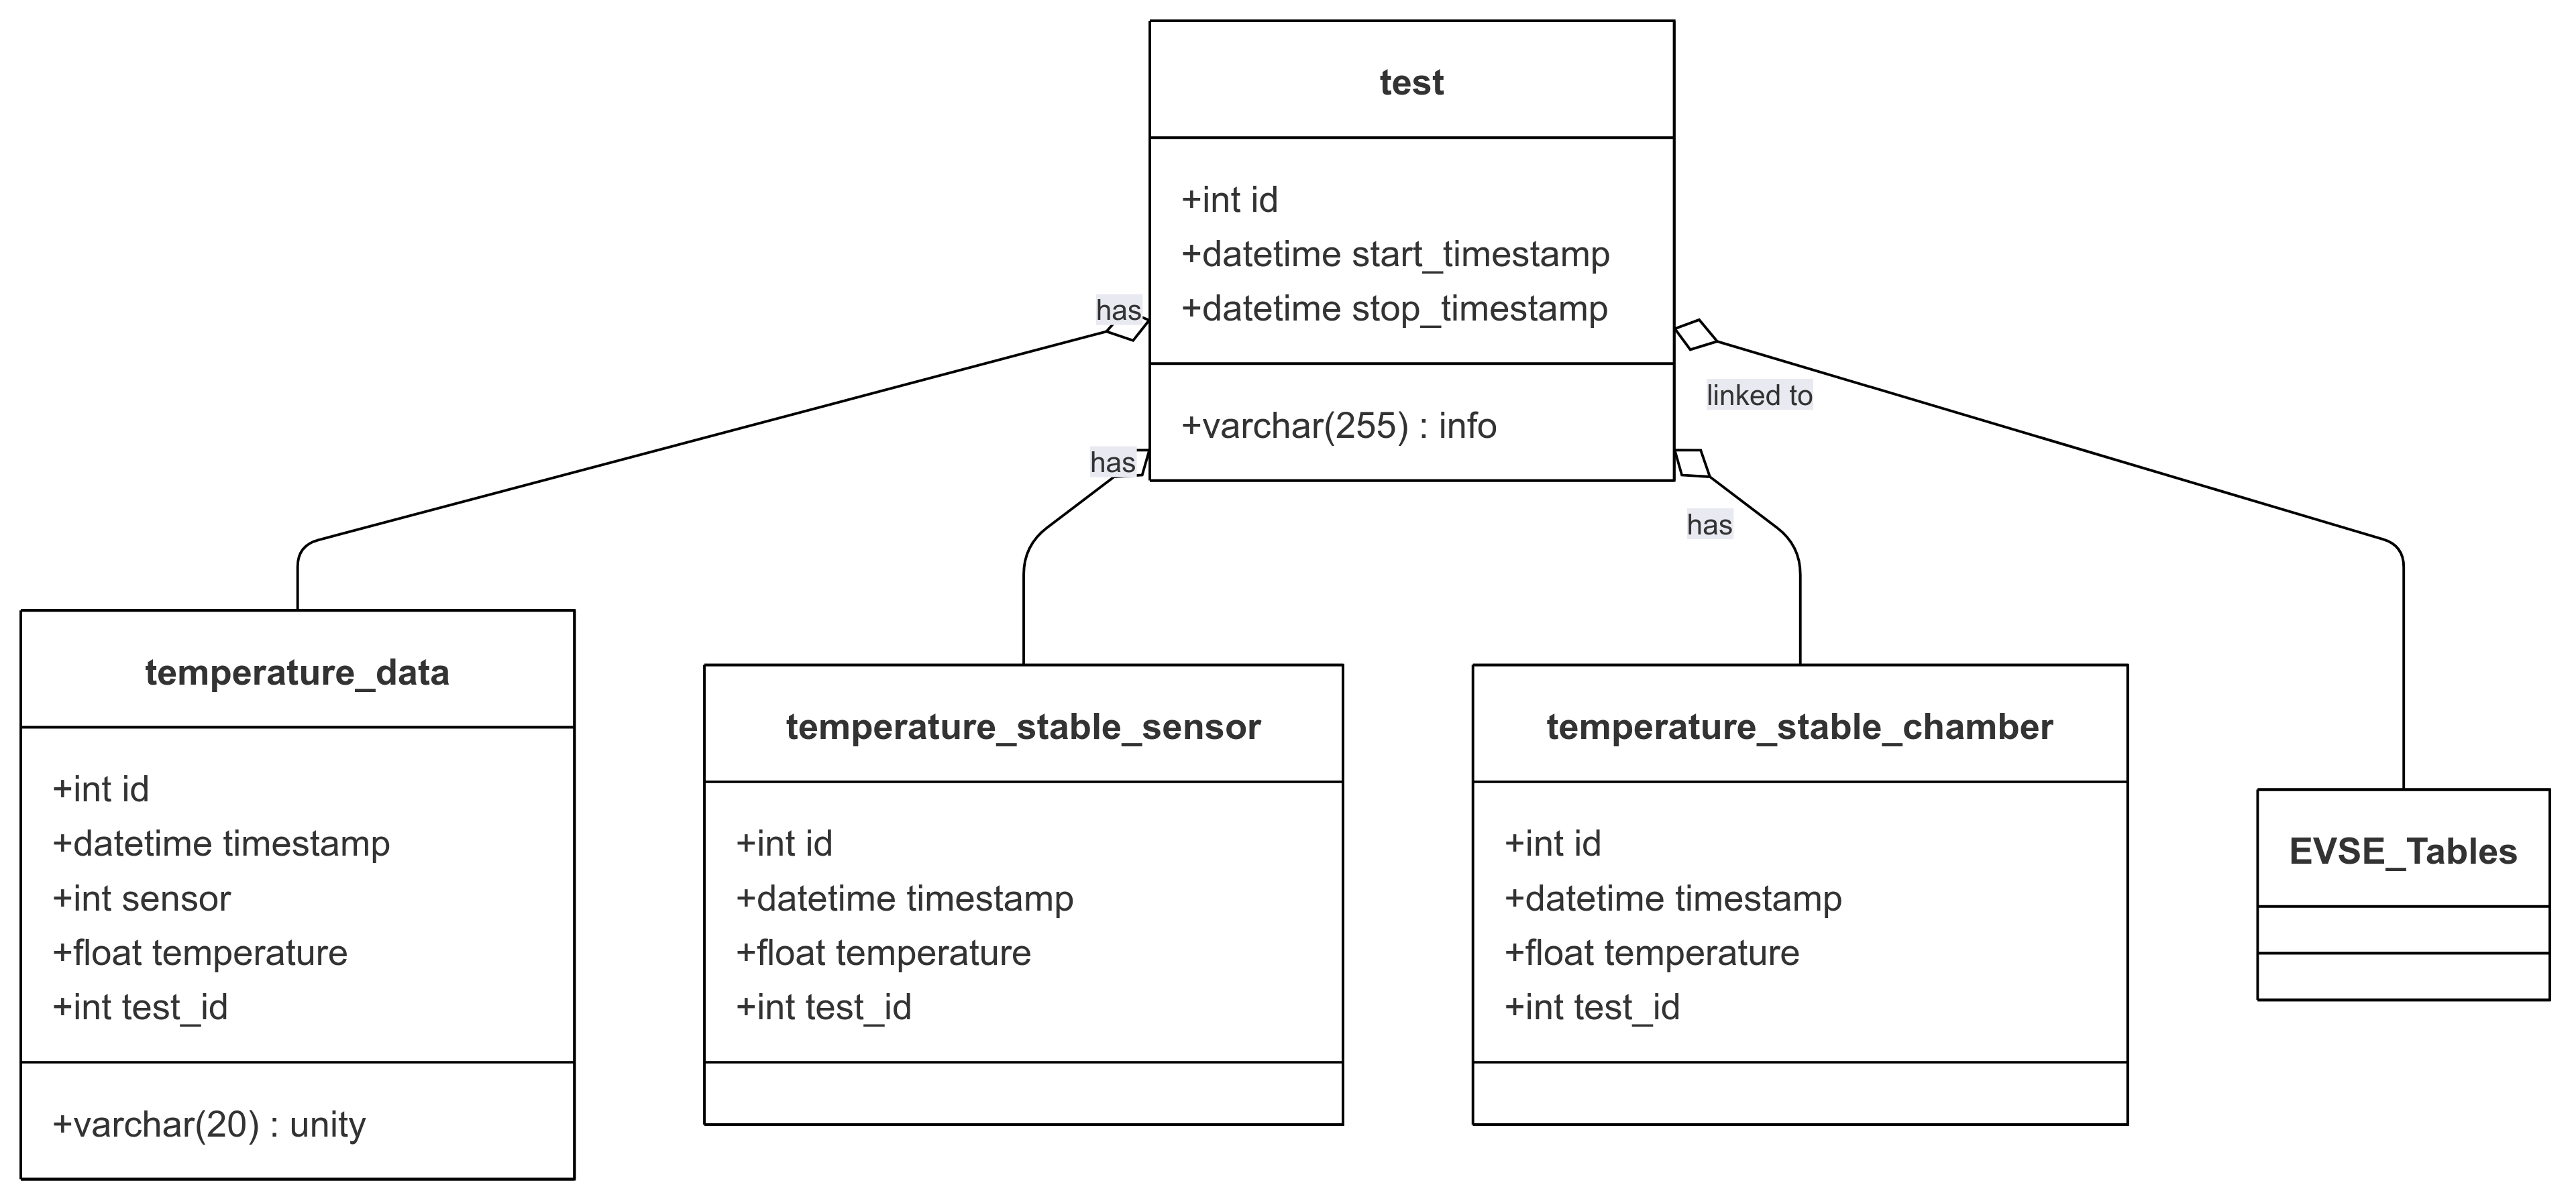
\includegraphics[width=\textwidth]{figures/class_diagram.png}
    \caption{Diagrama de classes da base de dados do protocolo}
    \label{fig:class_diagram}
\end{figure}

As base de dados são acedidas através de uma biblioteca de Python chamada MySQL Connector, que permite a conexão e manipulação dos 
dados da base de dados MySQL. A tabela test é a tabela principal que armazena os dados do teste de temperatura,
enquanto que a tabela $temperature_data$ é a tabela que armazena os dados de temperatura obtidos dos sensores DS18B20.
As tabelas $temperature_stable_sensor$ e $temperature_stable_chamber$ são tabelas auxiliares que armazenam o momento que a temperatura
lida pelo sensor de controlo e o sensor da câmara termal estabilizou, respetivamente.

\subsubsection{Migração de dados e scheduling}

Scheduling é um sistema de agendamento de tarefas que permite a execução de tarefas em momentos específicos ou em intervalos regulares.

Como os testes de temperatura podem durar várias horas, foi necessário implementar um sistema de migração de dados entre as três 
componentes do sistema (RPI, MainPC e EVSE), para permitir a visualização dos dados obtidos em tempo real. Para tal, é importante
garantir a sincronização entre os diferentes componentes através da comunicação entre eles. É utilizado um sistema de scheduling
através de threads para realizar a migração de dados entre as diferentes componentes do sistema.

O sistema de scheduling na RPI é responsável por obter os dados do EVSE. O sistema de scheduling no MainPC é responsável por
obter os dados da presentes na RPI (valores de temperatura dos sensores DS18B20, sensor de controlo da câmara termal e dados do EVSE).

Além disso, após a RPI notificar o MainPC que o sensor de controlo da câmara termal e o sensor de controlo estabilizaram, o sistema
de scheduling do MainPC é responsável na próxima trigger realizar a migração desses dados para a base de dados do MainPC.

\begin{figure}[H]
    \centering
    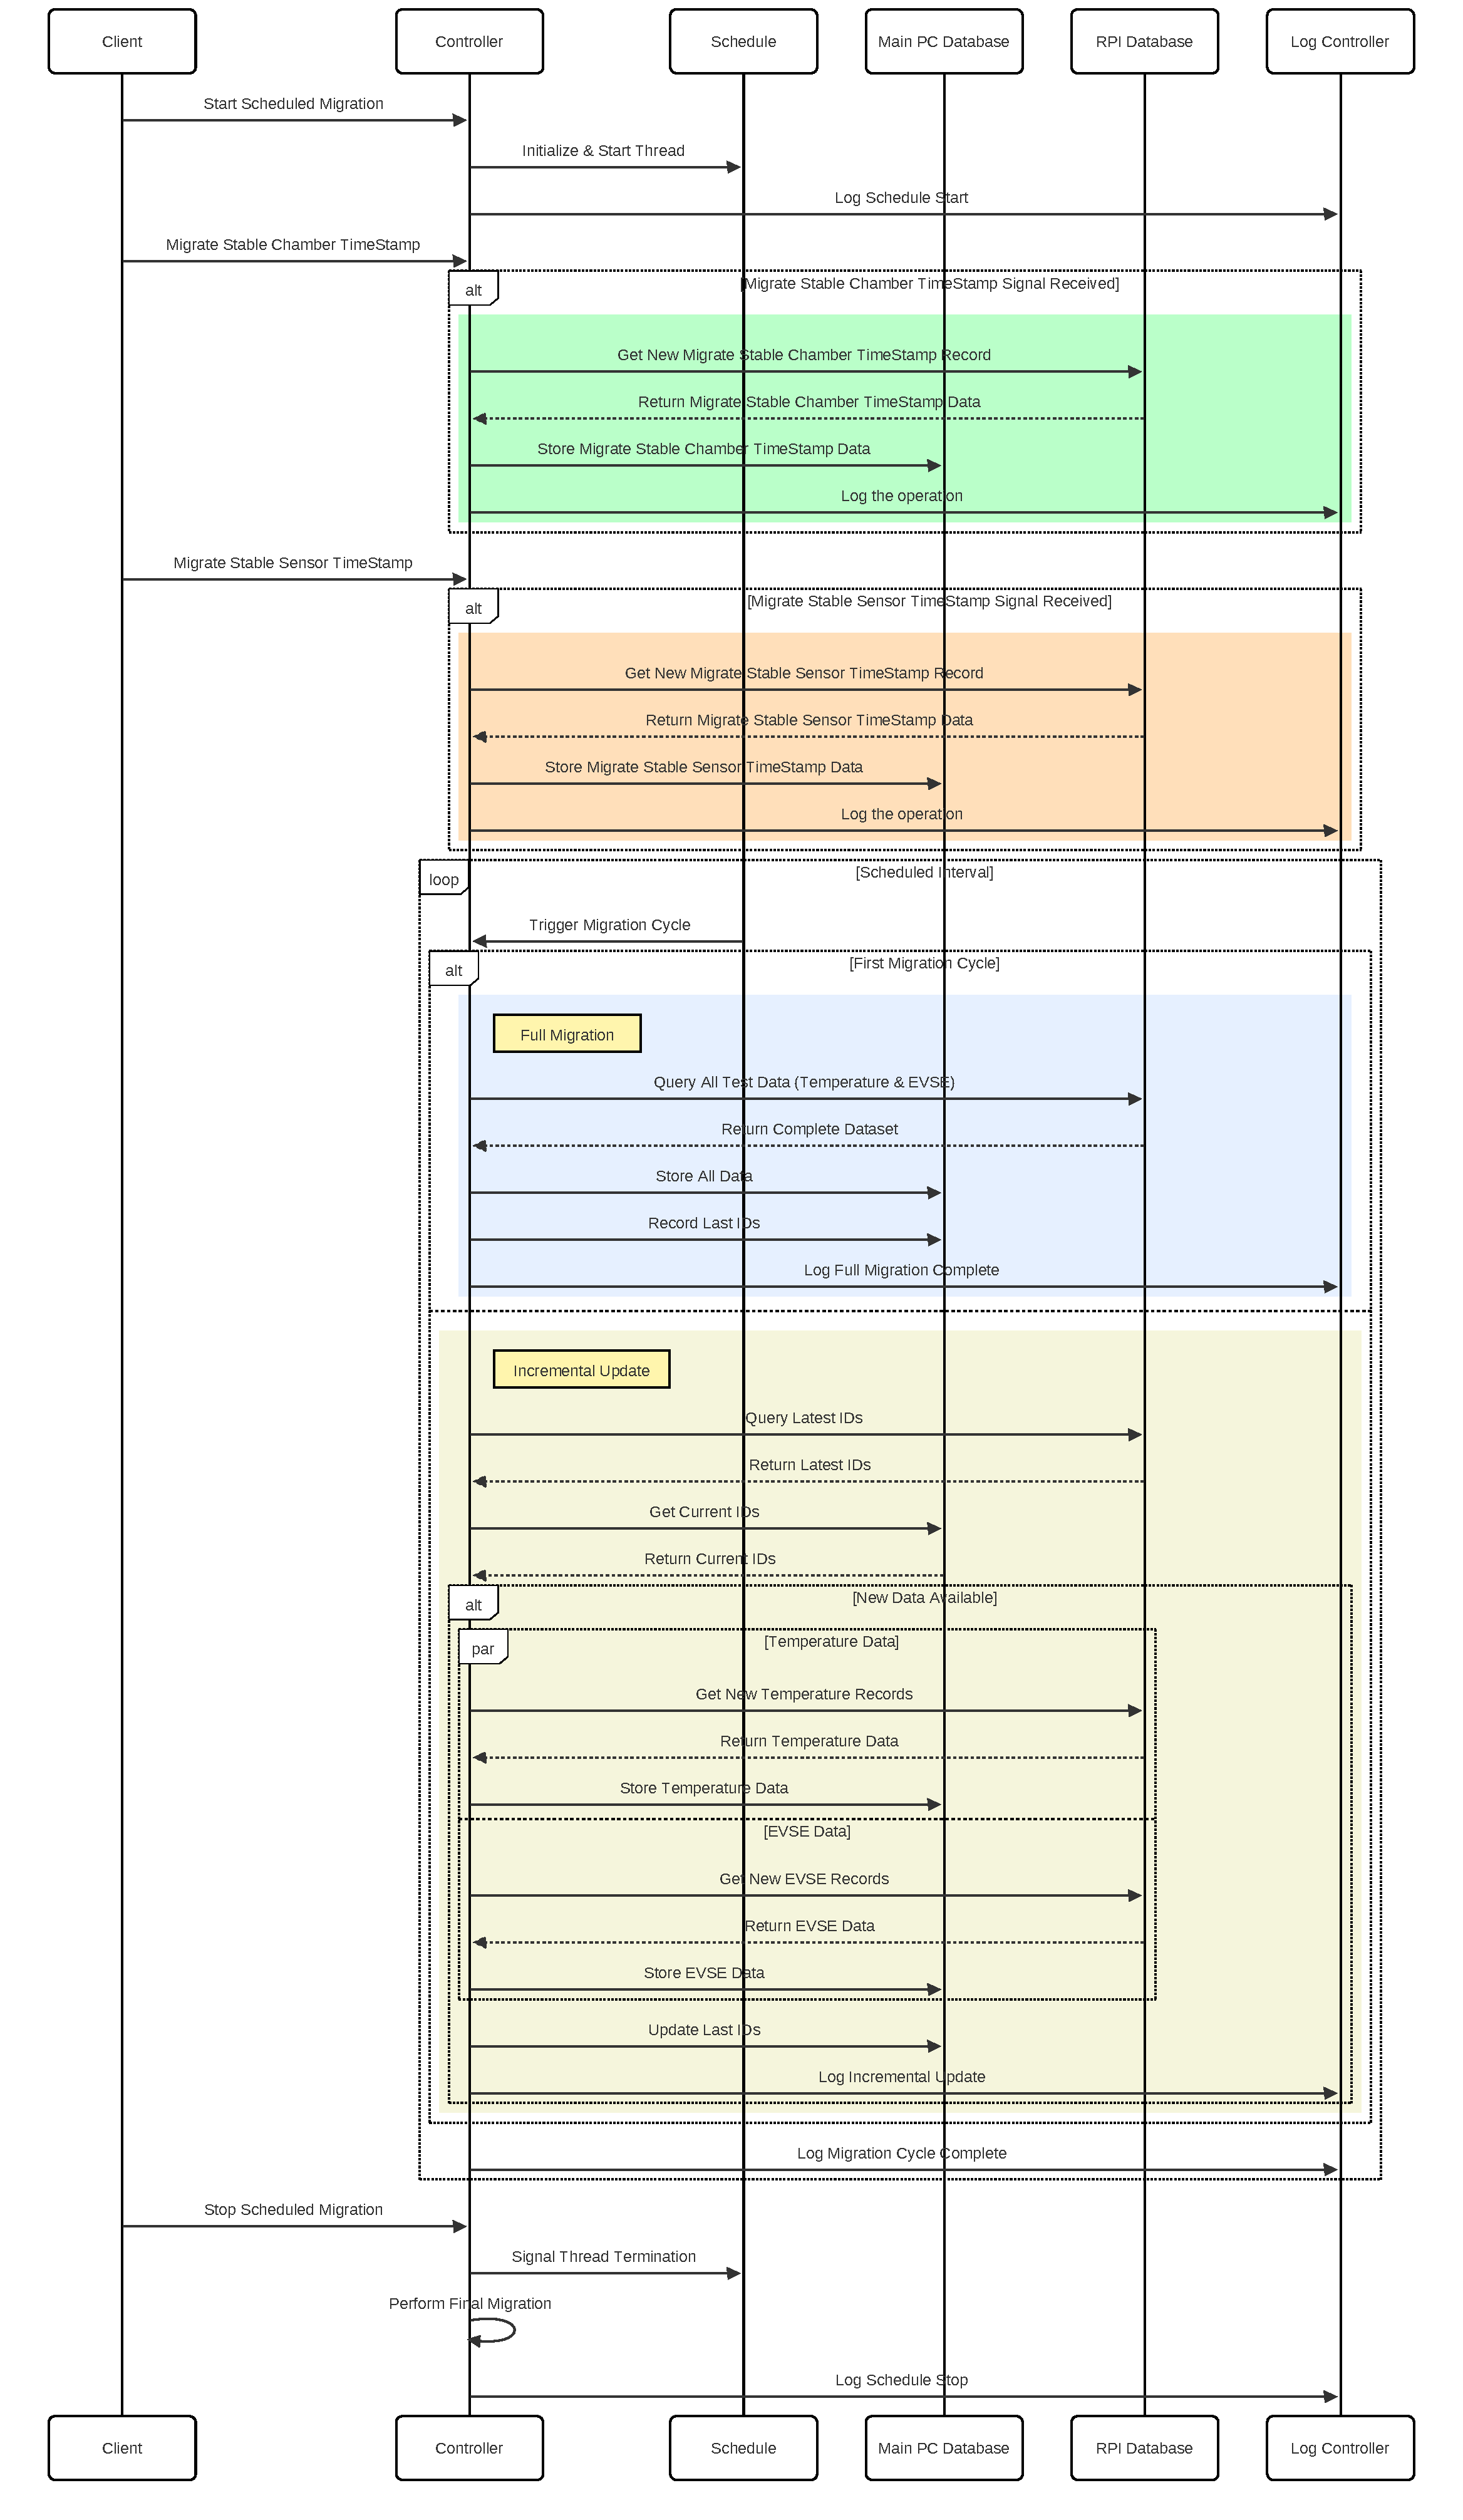
\includegraphics[scale=0.10]{figures/scheduling_1.pdf}
    \caption{Diagrama de sequência do sistema de scheduling do MainPC}
    \label{fig:scheduling_1}
\end{figure}

\begin{figure}[H]
    \centering
    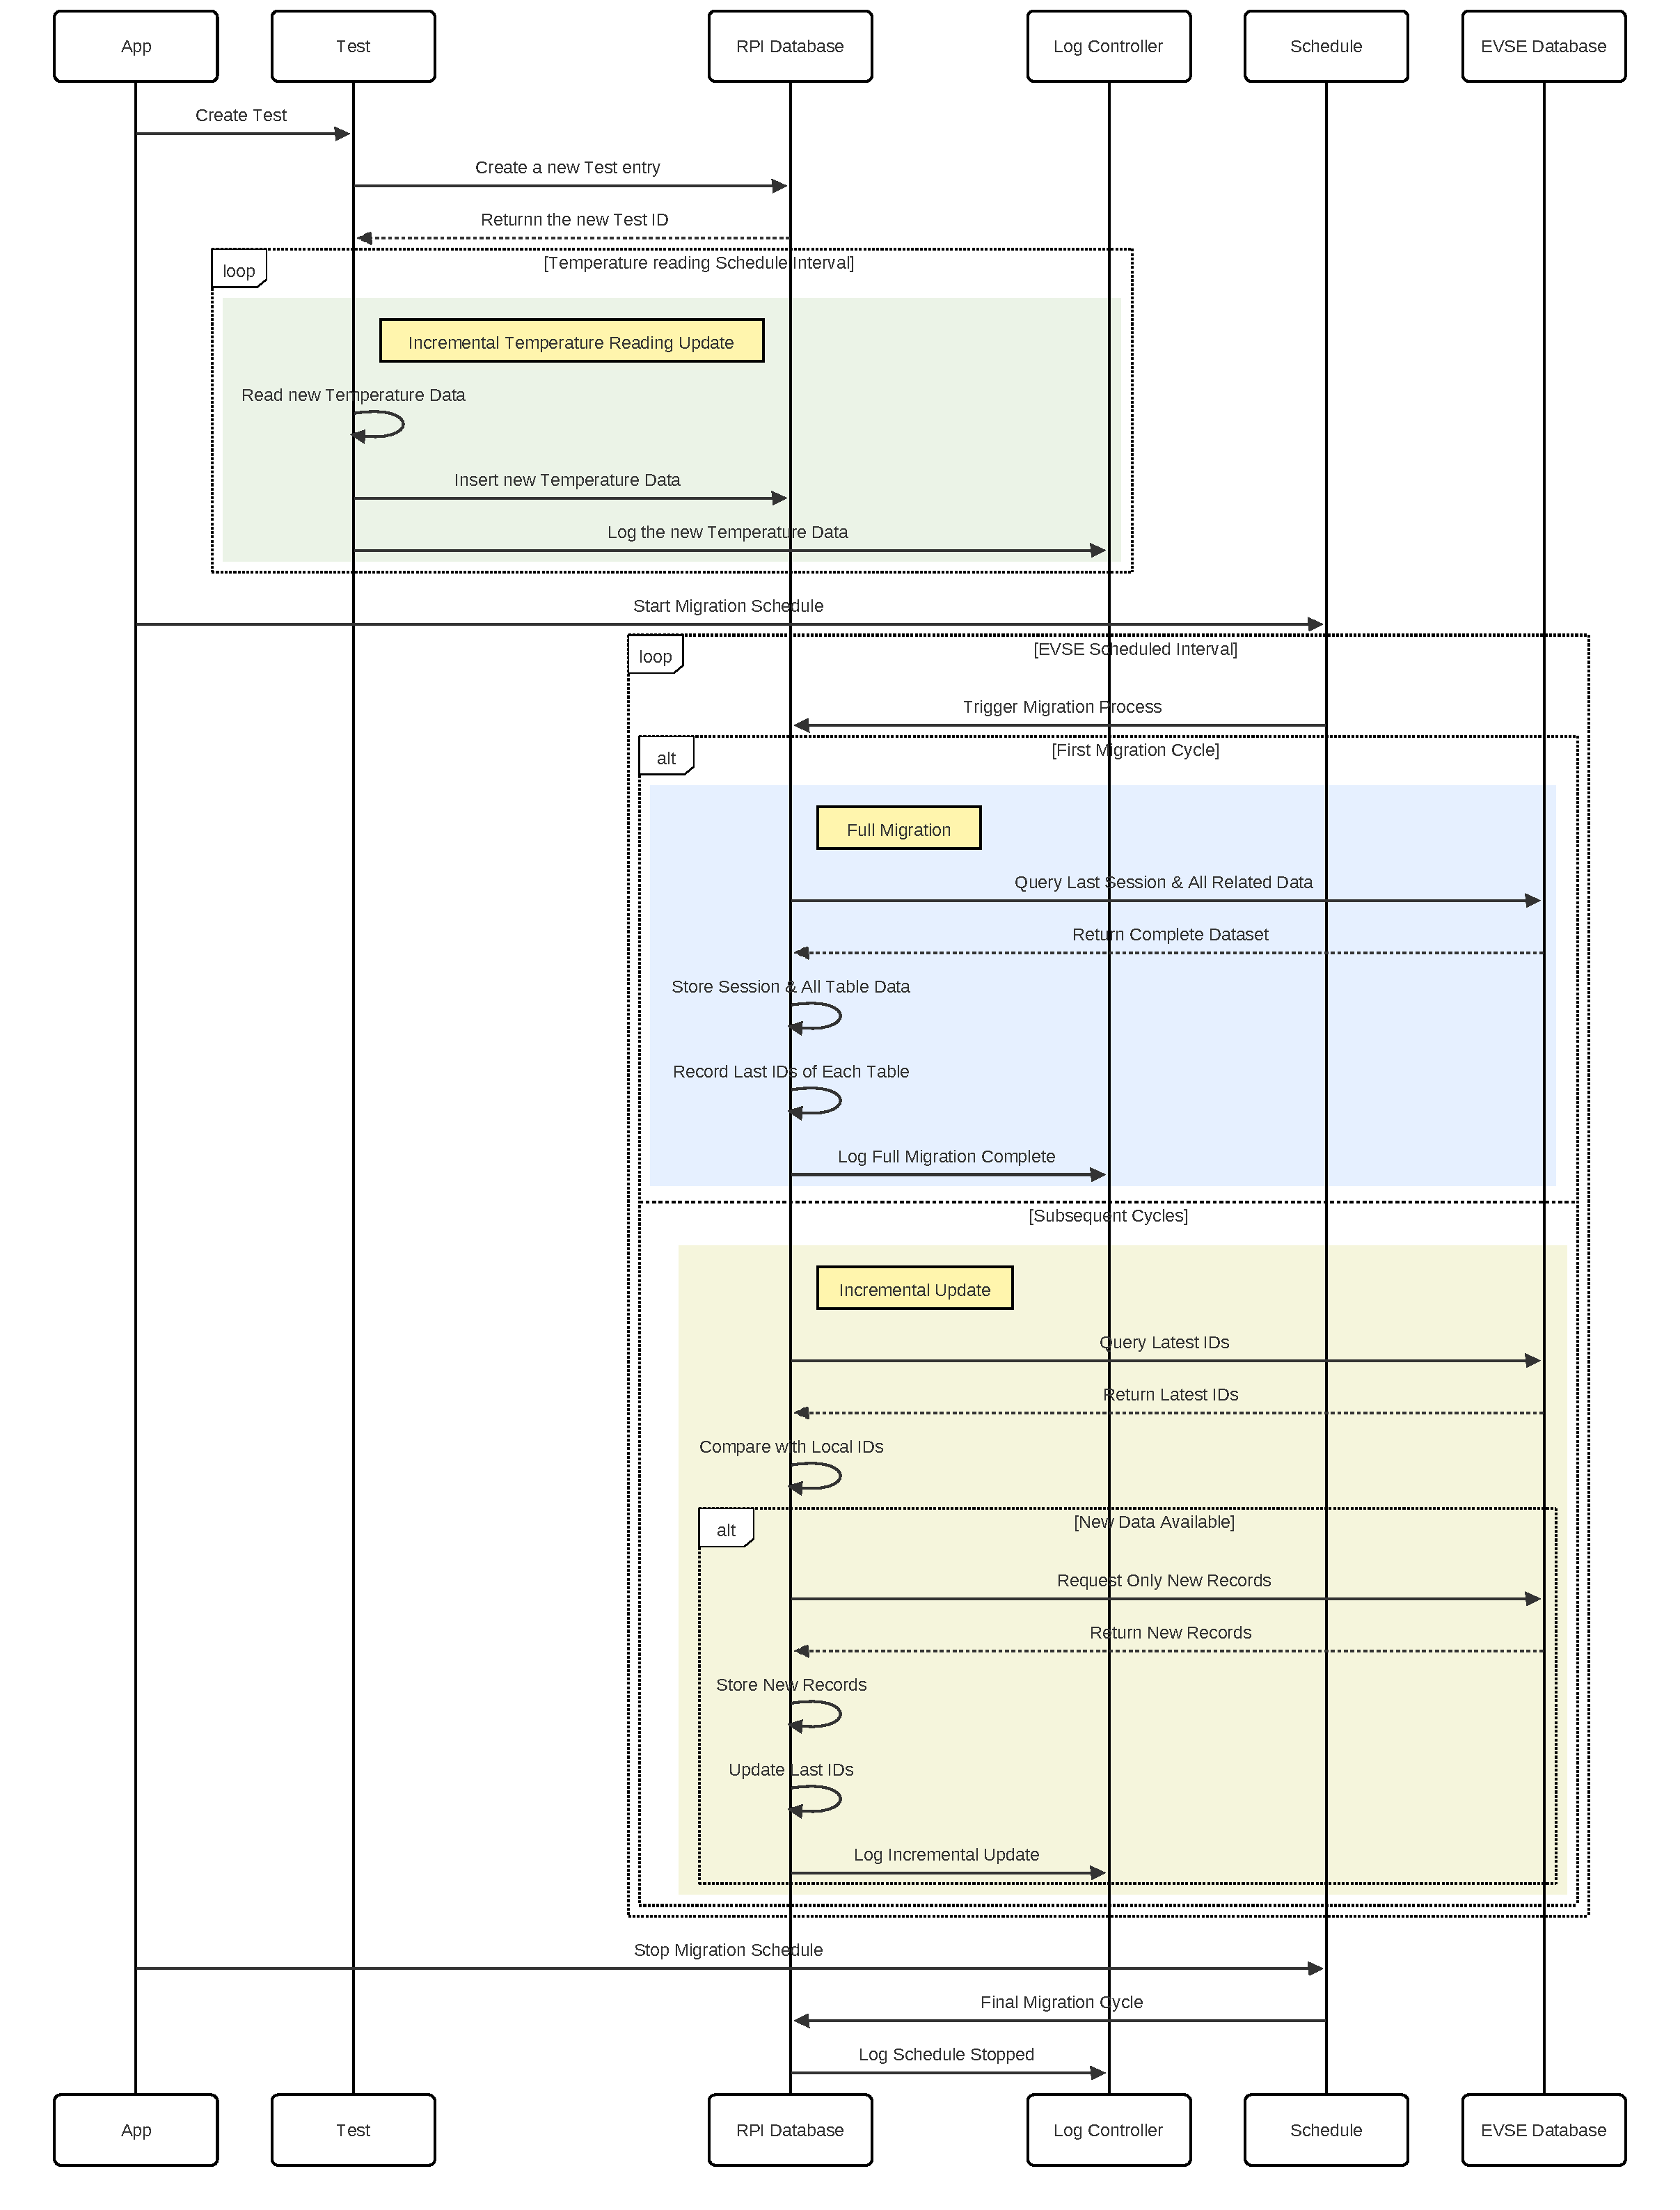
\includegraphics[scale=0.10]{figures/scheduling_2.pdf}
    \caption{Diagrama de sequência do sistema de scheduling da RPI}
    \label{fig:scheduling_2}
\end{figure}

\subsubsection{Dashboard}
Uma dashboard é uma interface gráfica que permite visualizar dados de uma forma interativa e personalizada. O objetivo principal da dashboard 
é permitir ao utilizador visualizar os dados obtidos do teste de temperatura em tempo real e do carregador em tempo real.

O Grafana não só permite a visualização dos dados obtidos em tempo real de forma gráfica, como também a criação automática de anotações
para mostar os momentos onde a temperatura estabelizou (tanto do sensor de controlo da câmara termal como do sensor de controlo do EVSE).

Além disso, é possível inserir o valor teórico de potência do carregador para calcular a eficiência do carregamento do carro elétrico
ao longo do tempo, permitindo uma análise mais detalhada do desempenho do carregamento.

Outro fator importante é a fácil troca de visualização dos testes, permitindo ao utilizador selecionar o teste que deseja visualizar e analisar os dados obtidos. 

\begin{figure}[H]
    \centering
    \begin{minipage}{0.8\textwidth}
        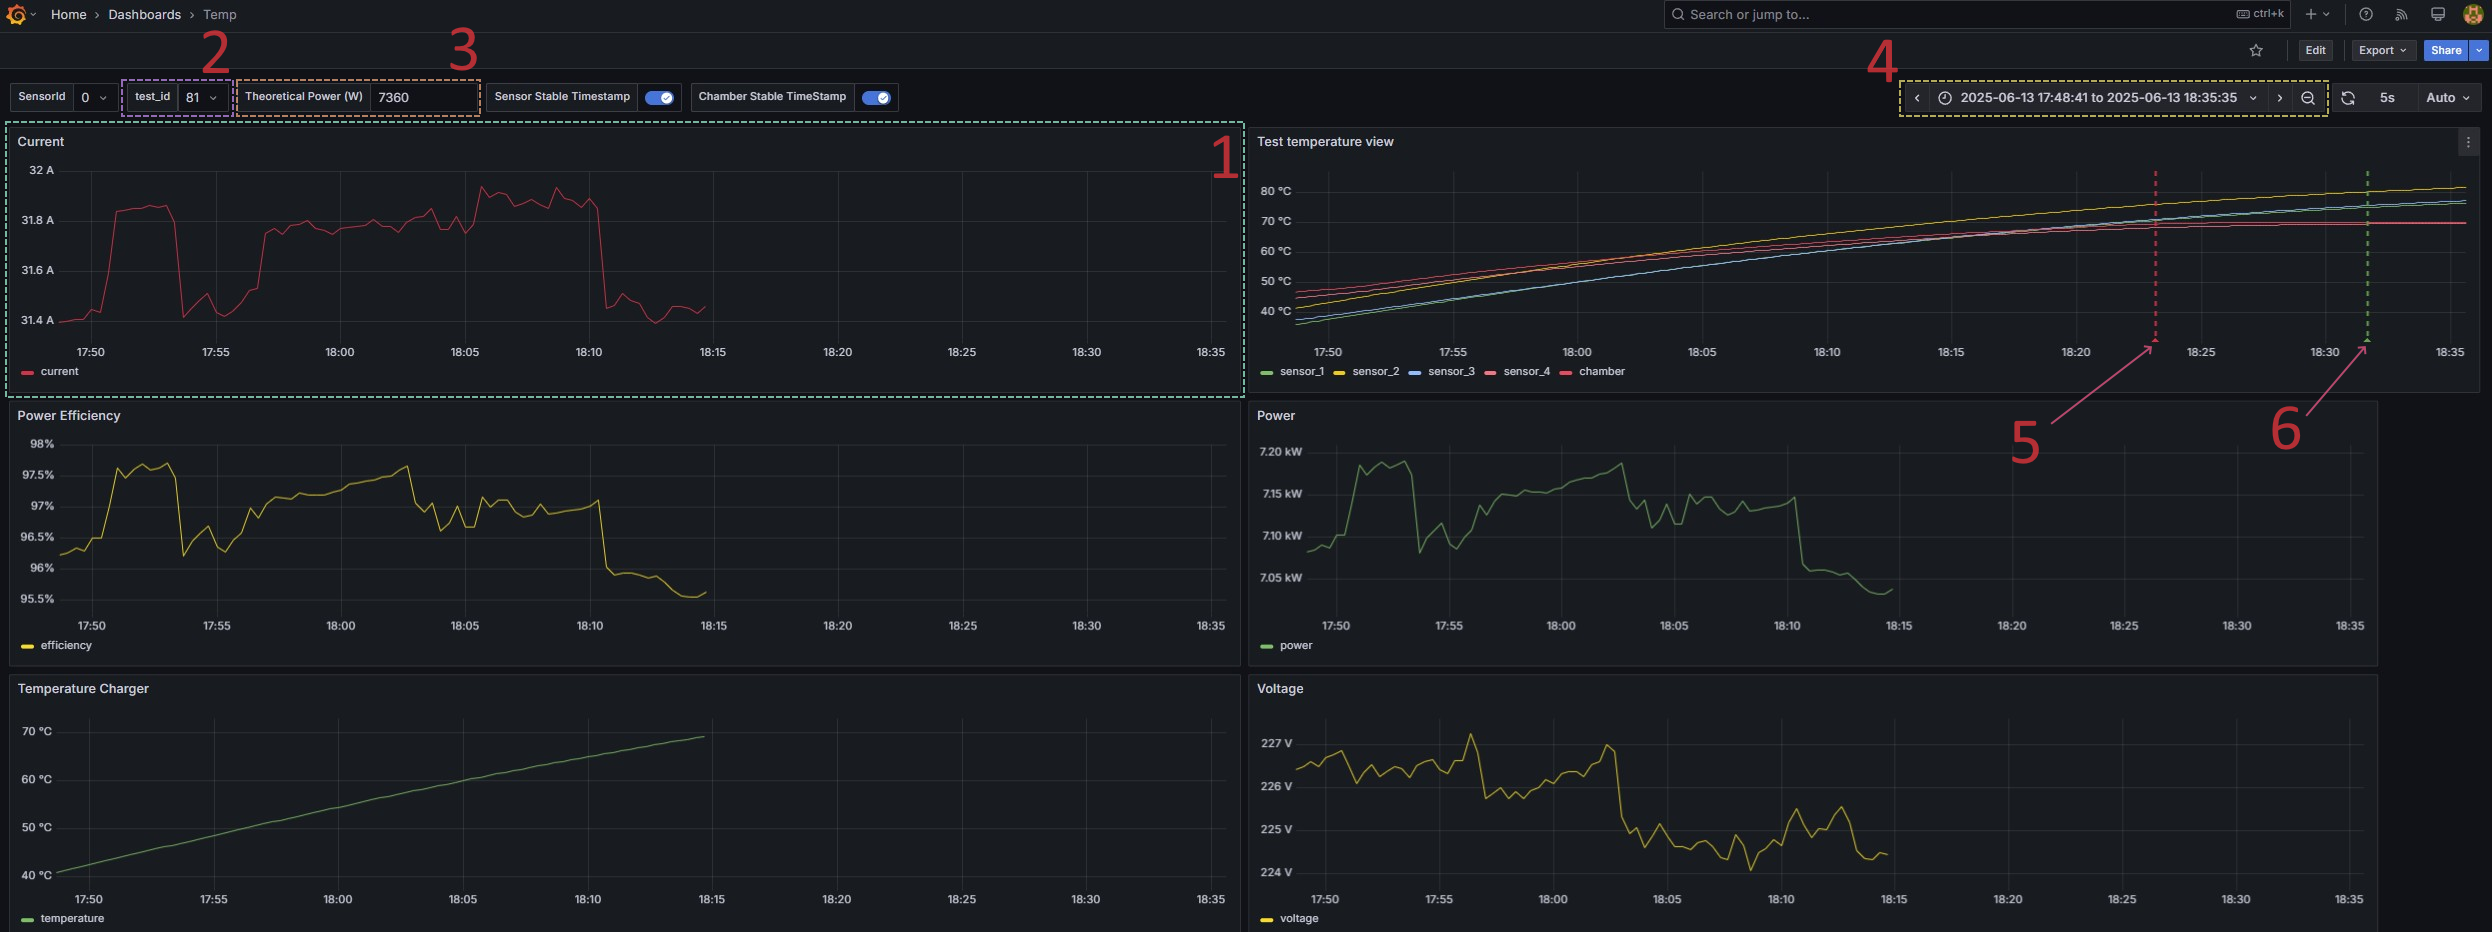
\includegraphics[width=\linewidth]{figures/dashboard.png}
    \end{minipage}
    \caption{Dashboard de visualização dos dados do teste}
    \label{fig:dashboard}
    
    \vspace{0.5em}
    \begin{minipage}{0.95\textwidth}
        \small
        \textbf{Legenda:}
        \begin{enumerate}
            \item Exemplo de gráfico de visualização dos dados obtidos do teste
            \item Dropdown de seleção do teste (via $test\_id$)
            \item Input box para o valor teórico de potência do carregador
            \item Seleção do intervalo de tempo para visualização dos dados
            \item Anotação automática de estabilização da temperatura do sensor da câmara termal
            \item Anotação automática de estabilização da temperatura do sensor de controlo
        \end{enumerate}
    \end{minipage}
\end{figure}

\subsubsection{Instalação e configuração}
Uma das tarefas desenvolvidas durante o estágio foi o Bootstrapping do sistema, para
permitir a sua rápida instalação e configuração. Para a instalação da componente RPI, foi utilizado um ansible
enquanto que para a instalação da componente MainPC foi utilizado um dockerfile com integração devcontainer
(mais informações na [DOCUMENTAÇÃO]).


Após o seu setup inicial e configuração do sistema, as diferentes componentes de hardware
têm que ser devidamente conectadas e posicionadas. Nas próximas figuras podem ser vista
a sua instalação (mais informações na [DOCUMENTAÇÃO]):

\begin{figure}[H]
    \centering
    \begin{minipage}{0.6\textwidth}
        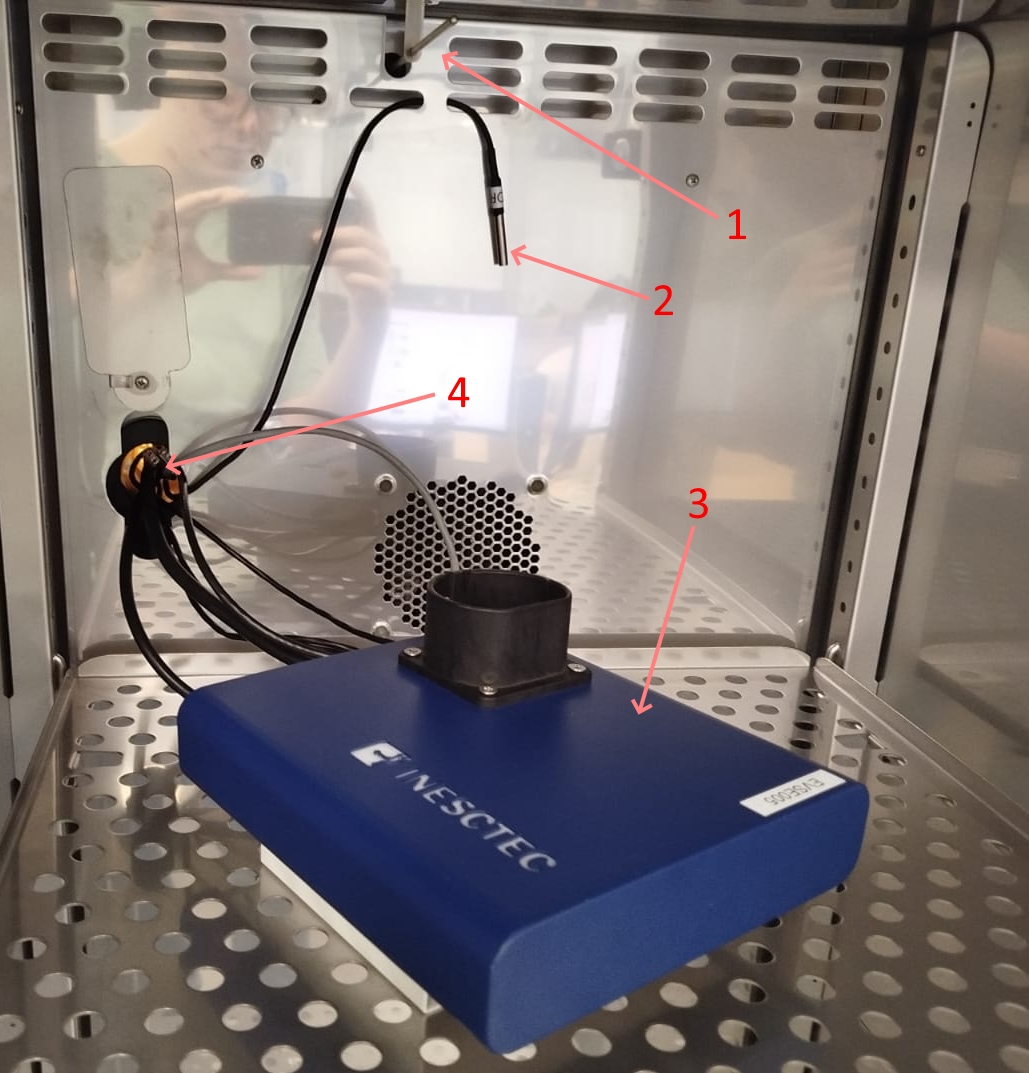
\includegraphics[width=\linewidth]{figures/inst_inside_1.png}
    \end{minipage}%
    \hfill
    \begin{minipage}{0.35\textwidth}
        \small
        \textbf{Legenda:}
        \begin{enumerate}
            \item Sensor da câmara termal
            \item Sensor DS18B20 de controlo da temperatura da câmara
            \item EVSE
            \item Entrada para o exterior da câmara termal
        \end{enumerate}
    \end{minipage}
    \caption{Imagem do EVSE dentro da câmara termal}
    \label{fig:inst_inside_1}
\end{figure}

\begin{figure}[H]
    \centering
    \begin{minipage}{0.6\textwidth}
        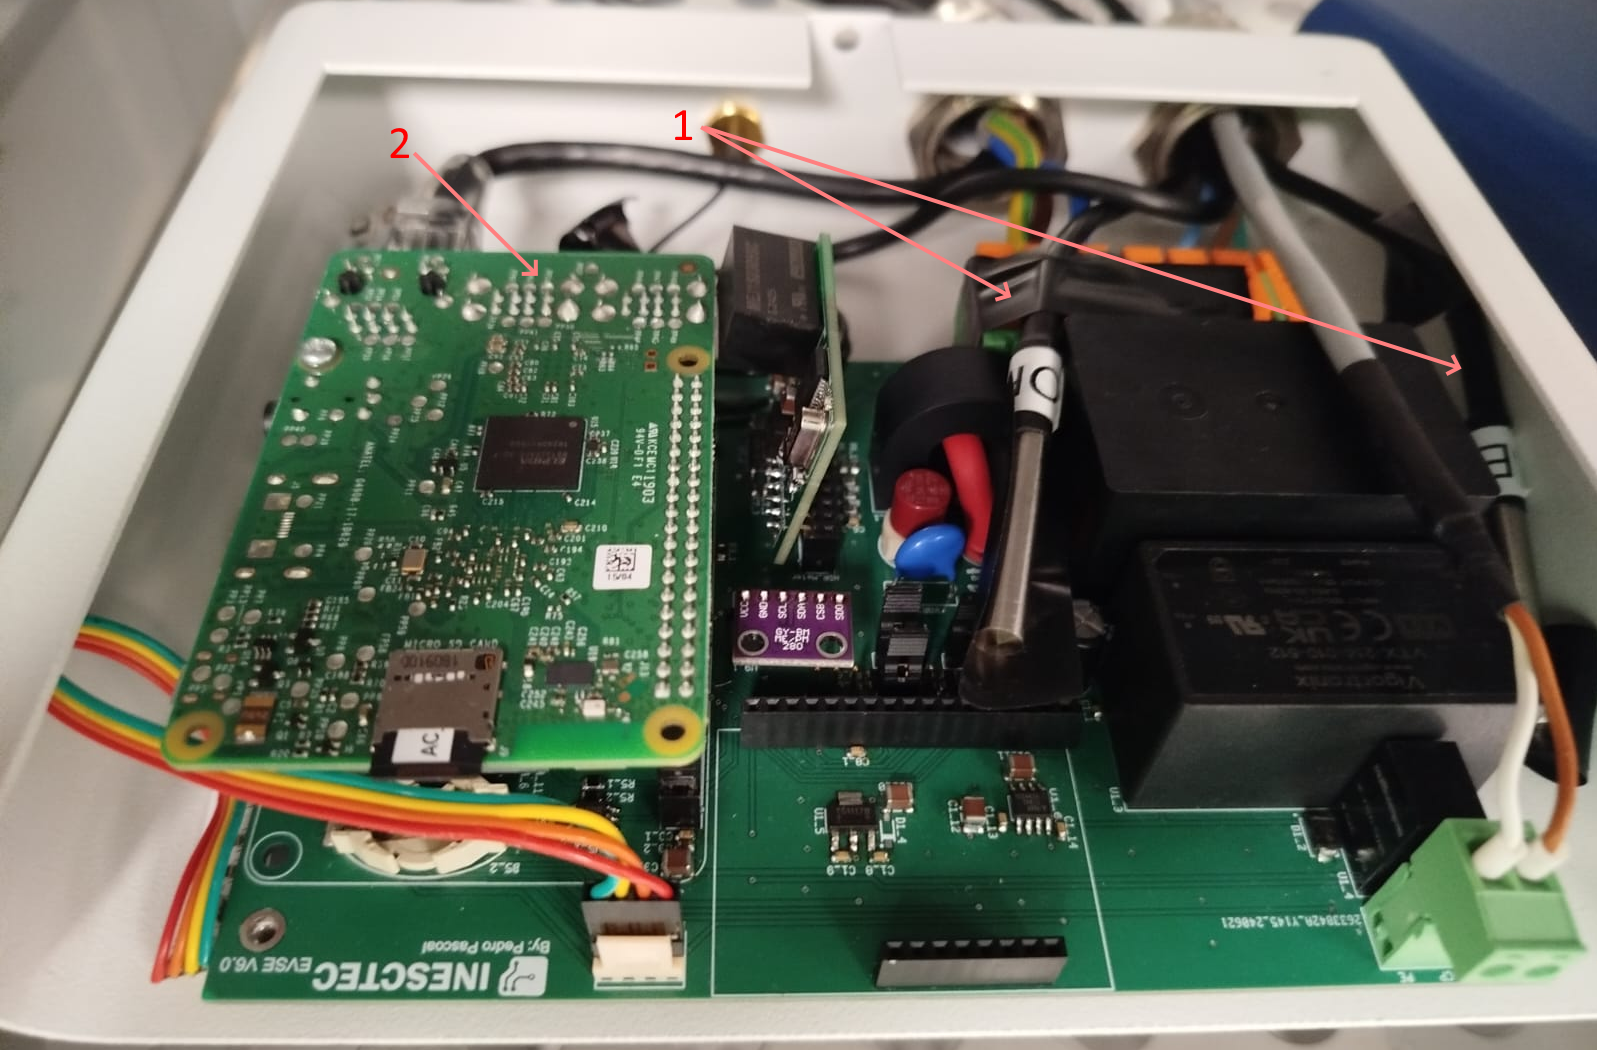
\includegraphics[width=\linewidth]{figures/inst_inside_2.png}
    \end{minipage}%
    \hfill
    \begin{minipage}{0.35\textwidth}
        \small
        \textbf{Legenda:}
        \begin{enumerate}
            \item Sensores DS18B20 posicionadas dentro do EVSE
            \item Raspberry do EVSE
        \end{enumerate}
    \end{minipage}
    \caption{Posicionamento dos sensores DS18B20 dentro do EVSE}
    \label{fig:inst_inside_2}
\end{figure}

\begin{figure}[H]
    \centering
    \begin{minipage}{0.6\textwidth}
        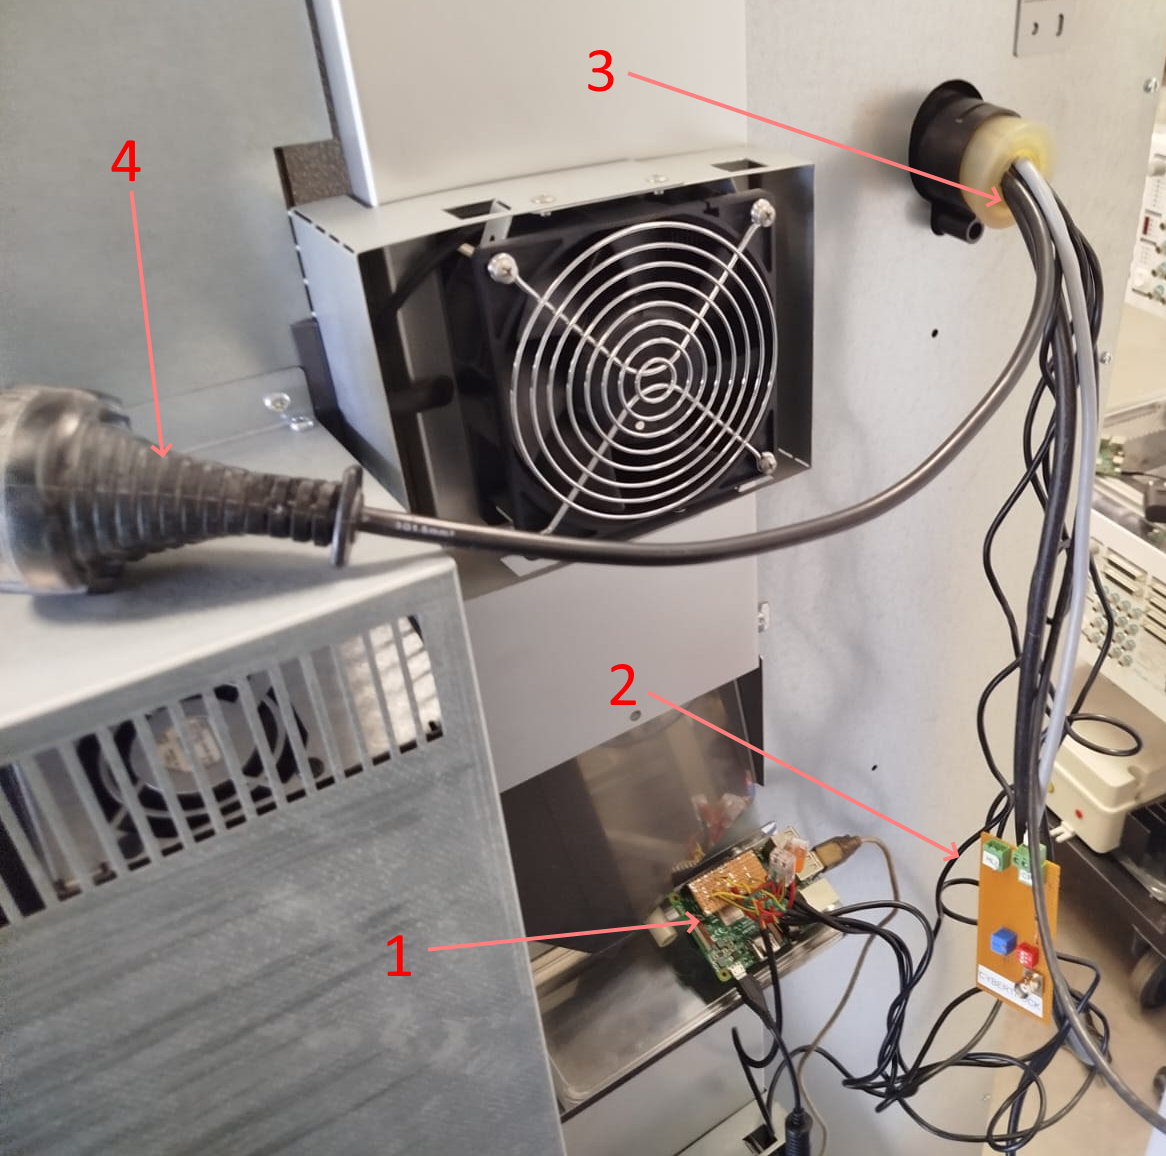
\includegraphics[width=\linewidth]{figures/inst_inside_3.png}
    \end{minipage}%
    \hfill
    \begin{minipage}{0.35\textwidth}
        \small
        \textbf{Legenda:}
        \begin{enumerate}
            \item RPI de controlo do teste
            \item ... TODO
            \item Entrada para o interior da câmara termal
            \item ... TODO
        \end{enumerate}
    \end{minipage}
    \caption{Parte externa traseira da câmara termal}
    \label{fig:inst_inside_3}
\end{figure}

\begin{figure}[H]
    \centering
    \begin{minipage}{0.6\textwidth}
        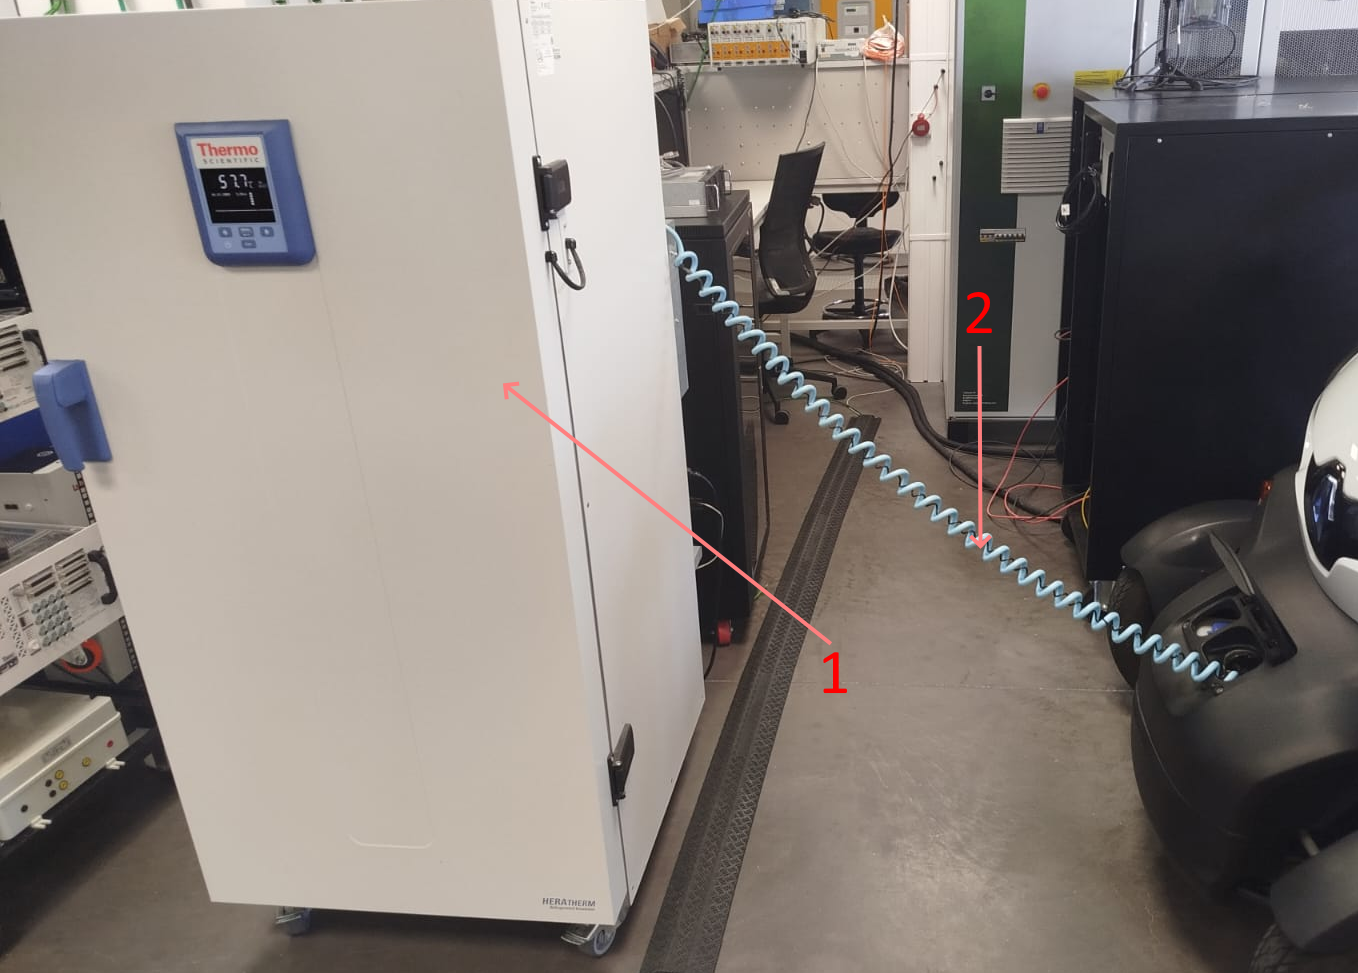
\includegraphics[width=\linewidth]{figures/inst_inside_4.png}
    \end{minipage}%
    \hfill
    \begin{minipage}{0.35\textwidth}
        \small
        \textbf{Legenda:}
        \begin{enumerate}
            \item Câmara termal IMP 400
            \item Cabo de carregamento do carro
        \end{enumerate}
    \end{minipage}
    \caption{Parte externa traseira da câmara termal}
    \label{fig:inst_inside_4}
\end{figure}

\subsection{Validação}

Para validação do protocolo foram realizados vários testes do mesmo ao longo do estágio. Os testes mais relevantes realizados
foram os seguintes:
\begin{itemize}
    \item Precisão e exatidão dos sensores DS18B20: Colocar os sensores DS18B20 dentro da câmara termal e verificar se os valores lidos pelos sensores são 
    coerentes com a temperatura da câmara termal (foram realizadas diversas iterações com diferentes temperaturas na 
    câmara);
    \item Schedulling: Verificar se o sistema de schedulling estar a funcionar corretamente com todas as componentes do
    sistema (MainPC, RPI e EVSE). Para tal foram colocados os sensores DS18B20 da camara termal enquanto o EVSE estava fora da câmara
    a enviar dados sem ter nenhum carregamento a decorrer;
    \item Logistica: Verificar a disposição de três sensores DS18B20 dentro do EVSE dentro da câmara termal. Também serviu
    para verificar a nossa hipotese de que o carregador estaria a uma temperatura inferior da câmara termal enquanto a temperatura
    da câmara termal não estivesse estabelizada (a aumentar a temperatura, por exemplo), mas que eventualmente o carregador iria atinjir uma 
    temperatura superior à da câmara termal;
    \item Teste com um carro elétrico: Para validar o protocolo em condições reais, foi realizado um teste com diferentes
    veículos elétricos que requerem diferentes potências de carregamento. Os resultados obtidos não só validaram o protocolo, como também
    permitiram verificar a eficiência do carregamento do carro elétrico ao longo do tempo.
\end{itemize}

Os resultados obtidos dos testes realizados em condições reais revelaram que o carregador EVSE em temperaturas altas (acima dos 60°C)
o carregador consegue manter a eficiencia de carregamento acima dos 95\% (o que é considerado aceitável para o carregamento de veículos elétricos).

(TODO adicionar mais informações sobre os testes realizados e os resultados obtidos)

